\documentclass{article}%
\usepackage[T1]{fontenc}%
\usepackage[utf8]{inputenc}%
\usepackage{lmodern}%
\usepackage{textcomp}%
\usepackage{lastpage}%
\usepackage[head=40pt,margin=0.5in,bottom=0.6in]{geometry}%
\usepackage{graphicx}%
%
\title{\textbf{Médicos y enfermeras del HUC protestan por tener cinco días sin agua}}%
\author{El Nacional Web}%
\date{24/09/2018}%
%
\begin{document}%
\normalsize%
\maketitle%
\textbf{URL: }%
http://www.el{-}nacional.com/noticias/protestas/medicos{-}enfermeras{-}del{-}huc{-}protestan{-}por{-}tener{-}cinco{-}dias{-}sin{-}agua\_252976\newline%
%
\textbf{Periodico: }%
EN, %
ID: %
252976, %
Seccion: %
Protestas\newline%
%
\textbf{Palabras Claves: }%
Salud, Caracas, Protestas, Sociedad\newline%
%
\textbf{Derecho: }%
2.1, %
Otros Derechos: %
, %
Sub Derechos: %
2.1.1\newline%
%
\textbf{EP: }%
SI\newline%
\newline%
%
\textbf{\textit{Mauro Zambrano, dirigente sindical de Fetrasalud, señaló que las intervenciones quirúrgicas y el servicio de diálisis fueron suspendidos en el hospital}}%
\newline%
\newline%
%
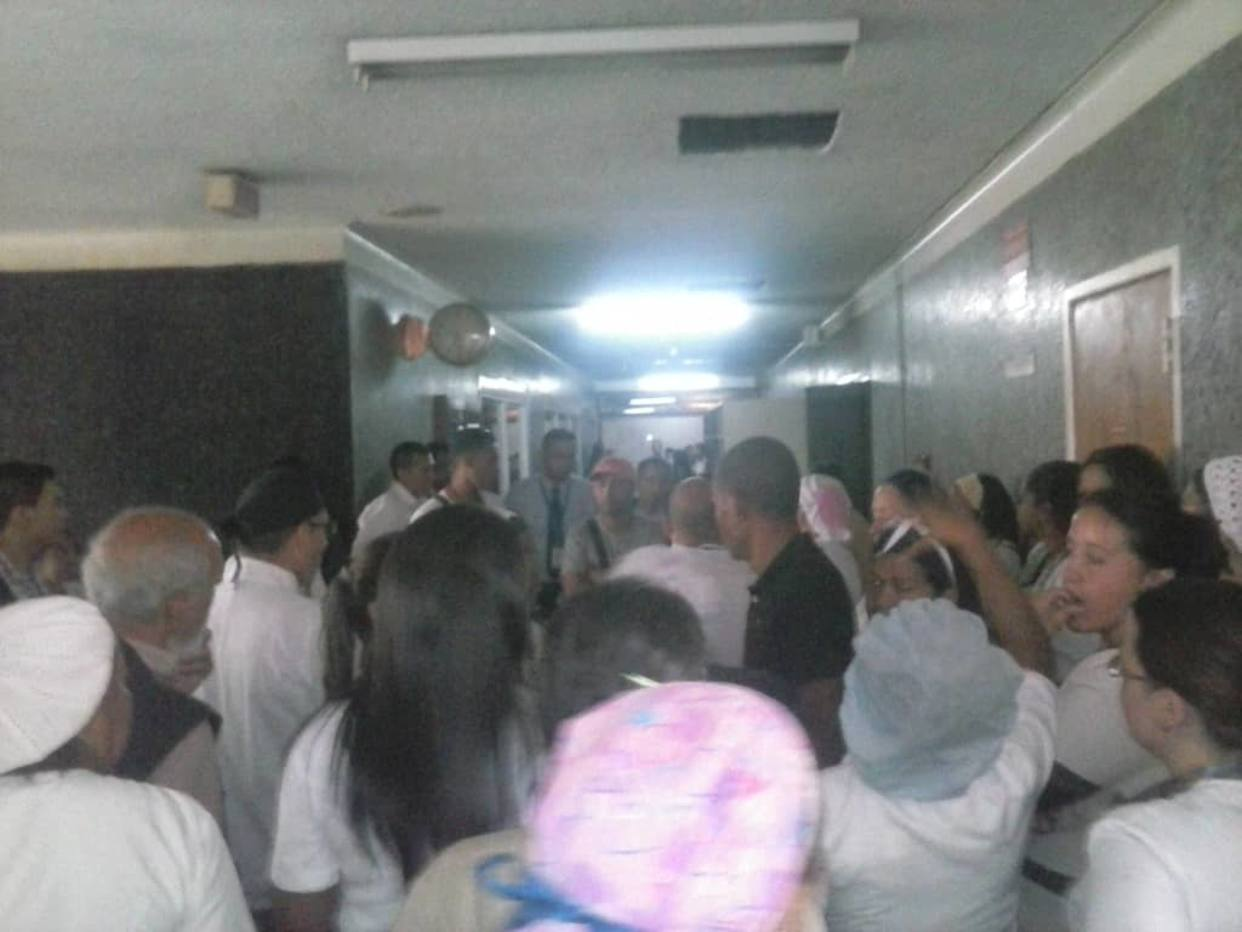
\includegraphics[width=300px]{47.jpg}%
\newline%
%
Médicos y enfermeras del Hospital Universitario de Caracas (HUC) protestan la mañana de este lunes luego de tener cinco días sin suministro de agua en el centro de salud.%
\newline%
%
Mauro Zambrano, dirigente sindical de Fetrasalud, denunció que la situación provocó la suspensión de las intervenciones quirúrgicas y el servicio de diálisis.%
\newline%
%
“Protesta. En el Hospital Universitario de Caracas tienen más de cinco días sin agua. Las intervenciones quirúrgicas y el servicio de diálisis están suspendidos”, explicó.%
\newline%
%
Zambrano también hizo una denuncia sobre la porción del desayuno que recibieron los pacientes que se encuentran en el HUC. En la imagen difundida por el dirigente se puede observar lo que parece ser una panqueca de pequeñas proporciones sobre una bandeja de metal.%
\newline%
%
\end{document}